\documentclass[a4paper]{article}
\usepackage[utf8]{inputenc} % para poder usar tildes en archivos UTF-8
\usepackage[spanish]{babel} % para que comandos como \today den el resultado en castellano
\usepackage{a4wide} % márgenes un poco más anchos que lo usual
\usepackage[showRevisiones]{caratula}
\usepackage{xcolor}
\usepackage{listings}
\lstset{basicstyle=\ttfamily,
  showstringspaces=false,
  commentstyle=\color{red},
  keywordstyle=\color{blue}
}

\begin{document}

\materia{Organización de Computadoras 66.20}
\tipoapunte{Trabajo Práctico #1}

\fecha{\today}

\autor{Quino López, Julián}{94224}{julian.quino2@gmail.com}
\autor{Del Carril, Manuel}{100772}{manueldelcarril@gmail.com}
\autor{Bobadilla Catalan, German}{90123}{bobadillagerman@gmail.com}

\revision{07/05/2019}{-}{Entrega del TP}

\maketitle

\renewcommand{\abstractname}{Resumen} 
\begin{abstract}
El siguiente trabajo práctico tiene como objetivo familiarizarse con el emulador GXEmul, que emula la arquitectura MIPS32, para lograr tal propósito se escribe en lenguaje C dos programas que permitan convertir archivos de texto desde Windows hacia UNIX y viceversa.
\end{abstract}


\section{Introducción}
Los archivos de texto requieren de un carácter especial (o secuencia de caracteres) para indicar el fin de una línea. La codificación de este varía según el sistema operativo, lo que lleva a la incorrecta visualización de un archivo en un sistema operativo que fue creado en otro. Linux utiliza el salto de línea \verb|(\n)| mientras que Windows utiliza el retorno del carro seguido del salto de línea \verb|(\r\n)|.

\section{Desarrollo}

El algoritmo propuesto por el grupo consiste en recorrer caracter por caracter hasta encontrar un \verb|\r|, si el programa usado es dos2unix y el siguiente caracter es un \verb|\n| se elimnara el \verb|\r| , si en cambio se usa el programa unix2dos se agregara \verb|\r| antes de un \verb|\n|, esto se realiza ya sea desde el archivo o utilizando el stream leído por entrada standard.


\subsection{Comandos para compilar y ejecutar el programa}

Se puede compilar los programas con los siguientes comandos:

\begin{lstlisting}[language=bash]
  $ gcc unix2dos.c -o unix2dos
  $ gcc dos2unix.c -o dos2unix
\end{lstlisting}


Y luego ejecutarlos con los comandos:

\begin{lstlisting}[language=bash]
  $ ./unix2dos -i input.txt -o output.txt
  $ ./dos2unix -i input.txt -o output.txt
\end{lstlisting}

En caso de sólo querer especificar el archivo de entrada, debe ejecutarse, por ejemplo, de la siguiente manera:

\begin{lstlisting}[language=bash]
  $ ./unix2dos -i input.txt -o -
  $ ./dos2unix -i input.txt -o -
\end{lstlisting}

Análogamente si se quiere ingresar un archivo de salida:

\begin{lstlisting}[language=bash]
  $ ./unix2dos -i - -o output.txt
  $ ./dos2unix -i - -o output.txt
\end{lstlisting}

Es decir que con un guión medio indicamos que no se proporcionará un archivo para entrada/salida, acorde a lo que indica el enunciado.

\subsection{Otros comandos}

Pueden utilizarse comandos tales como help y version, de la siguiente forma:

\begin{lstlisting}[language=bash]
  $ ./unix2dos -h
  $ ./dos2unix -h
\end{lstlisting}

\begin{lstlisting}[language=bash]
  $ ./unix2dos -V
  $ ./dos2unix -V
\end{lstlisting}

\subsection{Código fuente de unix2dos.c}
\lstset{breaklines=true}
\begin{lstlisting}[language=C]
#include <stdio.h>
#include <string.h>
#include <getopt.h>
#include <stdlib.h>
#include <unistd.h>
#include <errno.h>

#define ERROR -1
#define SALIDA_EXITOSA 0


/**
 * Procesa el archivo de entrada o el stream ingresado por stdin
 *
 * @param inputFile
 * @param outputFile
 * @return un código
 */
int processInput(FILE *inputFile, FILE *outputFile) {
    int c;
    while((c=fgetc(inputFile))!=EOF){
        if(c=='\r'){
            if((c=fgetc(inputFile))=='\n'){
            	fprintf(outputFile,"\r\n");
            }else{
            	fprintf(outputFile,"\r");
            }
        }else if(c=='\n'){
        	fprintf(outputFile,"\r\n");
        }
        else{
            fprintf(outputFile,"%c",c);
        }
    }
    if(fclose(inputFile)==EOF){
        fprintf(stderr, "Error fclose: %s\n", strerror( errno ));
        return ERROR;
    }
    if(outputFile != stdout){
        if(fclose(outputFile)==EOF){
            fprintf(stderr, "Error fclose: %s\n", strerror( errno));
            return ERROR;
        }
    }
    return SALIDA_EXITOSA;
}

int main(int argc, char *argv[]) {
    int option = 0;
    const char *short_opt = "i:o:hV";
    struct option long_opt[] = {
            {"version", no_argument,       NULL, 'V'},
            {"help",    no_argument,       NULL, 'h'},
            {"input",   required_argument, NULL, 'i'},
            {"output",  required_argument, NULL, 'o'},
            {NULL, 0,                      NULL, 0}
    };
    FILE *inputFile = NULL;
    FILE *outputFile = NULL;

    while ((option = getopt_long(argc, argv, short_opt, long_opt, NULL)) != -1) {
        switch (option) {
            case 'V':
                printf("TP #0 de la materia Organización de Computadoras \n");
                printf("Alumnos: \n");
                printf("	Bobadilla Catalan German\n	Del Carril Manuel \n	Quino Lopez Julian \n");
                return 0;
            case 'h':
                printf("Usage: \n");
                printf("	%s -h \n", argv[0]);
                printf("	%s -V \n", argv[0]);
                printf("	%s [options] \n", argv[0]);
                printf("Options: \n");
                printf("	-V, --version  Print version and quit. \n");
                printf("	-h, --help     Print this information. \n");
                printf("	-o, --output   Location of the output file. \n");
                printf("	-i, --input    Location of the input file. \n");
                return 0;
            case 'i':
            	if(strcmp(optarg, "-") != 0){
            		inputFile = fopen(optarg, "r");
            		if(inputFile == NULL){
            			fprintf(stderr, "Error archivo entrada: %s\n", strerror(errno));
            			return ERROR;
            		}
            	}
                break;
            case 'o':
            	if(strcmp(optarg, "-") != 0){
            		outputFile = fopen(optarg, "w+");
            		if(outputFile == NULL) {
            			fprintf(stderr, "Error archivo salida: %s\n", strerror(errno));
            			return ERROR;
            		}
            	}
                break;
            default:
                // asi esta en el manual de getopt
                abort();
        }
    }

    if(inputFile == NULL) {
        inputFile = stdin;
    }
    if(outputFile == NULL) {
        outputFile = stdout;
    }
    if(processInput(inputFile, outputFile) == ERROR) {
    	return ERROR;
    }
    return SALIDA_EXITOSA;
}

\end{lstlisting}

\subsection{Código fuente de dos2unix.c}
\begin{lstlisting}[language=C]

#include <stdio.h>
#include <string.h>
#include <getopt.h>
#include <stdlib.h>
#include <unistd.h>
#include <errno.h>

#define ERROR -1
#define SALIDA_EXITOSA 0


/**
 * Procesa el archivo de entrada o el stream ingresado por stdin
 *
 * @param inputFile
 * @param outputFile
 * @return un código
 */
int processInput(FILE *inputFile, FILE *outputFile) {
    int c;
    while((c=fgetc(inputFile))!=EOF){
        if(c=='\r'){
        	if((c=fgetc(inputFile))=='\n'){
        		fprintf(outputFile,"\n");
        	}
        	else{
        		fprintf(outputFile,"\r");
        		fprintf(outputFile,"%c",c);
        	}
        }
        else{
            fprintf(outputFile,"%c",c);
        }
    }
    if(fclose(inputFile)==EOF){
        fprintf(stderr, "Error fclose: %s\n", strerror( errno ));
        return ERROR;
    }
    if(outputFile != stdout){
        if(fclose(outputFile)==EOF){
            fprintf(stderr, "Error fclose: %s\n", strerror( errno));
            return ERROR;
        }
    }
    return SALIDA_EXITOSA;
}

int main(int argc, char *argv[]) {
    int option = 0;
    const char *short_opt = "i:o:hV";
    struct option long_opt[] = {
            {"version", no_argument,       NULL, 'V'},
            {"help",    no_argument,       NULL, 'h'},
            {"input",   required_argument, NULL, 'i'},
            {"output",  required_argument, NULL, 'o'},
            {NULL, 0,                      NULL, 0}
    };
    FILE *inputFile = NULL;
    FILE *outputFile = NULL;

    while ((option = getopt_long(argc, argv, short_opt, long_opt, NULL)) != -1) {
        switch (option) {
            case 'V':
                printf("TP #0 de la materia Organización de Computadoras \n");
                printf("Alumnos: \n");
                printf("	Bobadilla Catalan German\n	Del Carril Manuel \n	Quino Lopez Julian \n");
                return 0;
            case 'h':
                printf("Usage: \n");
                printf("	%s -h \n", argv[0]);
                printf("	%s -V \n", argv[0]);
                printf("	%s [options] \n", argv[0]);
                printf("Options: \n");
                printf("	-V, --version  Print version and quit. \n");
                printf("	-h, --help     Print this information. \n");
                printf("	-o, --output   Location of the output file. \n");
                printf("	-i, --input    Location of the input file. \n");
                return 0;
            case 'i':
            	if(strcmp(optarg, "-") != 0){
            		inputFile = fopen(optarg, "r");
            		if(inputFile == NULL) {
            			fprintf(stderr, "Error archivo entrada: %s\n", strerror(errno));
            			return ERROR;
            		}
            	}
                break;
            case 'o':
            	if(strcmp(optarg, "-") != 0){
            		outputFile = fopen(optarg, "w+");
            		if(outputFile == NULL) {
            			fprintf(stderr, "Error archivo salida: %s\n", strerror(errno));
            			return ERROR;
            		}
            	}
                break;
            default:
                // asi esta en el manual de getopt
                abort();
        }
    }
    if(inputFile == NULL) {
        inputFile = stdin;
    }
    if(outputFile == NULL) {
        outputFile = stdout;
    }
    if(processInput(inputFile, outputFile) == ERROR) {
    	return ERROR;
    }
    return SALIDA_EXITOSA;
}

\end{lstlisting}

\section{Casos de prueba}

A continuación se muestran unos casos de prueba desde la consola del GXEmul.


\begin{figure}[!htp]
\begin{center}
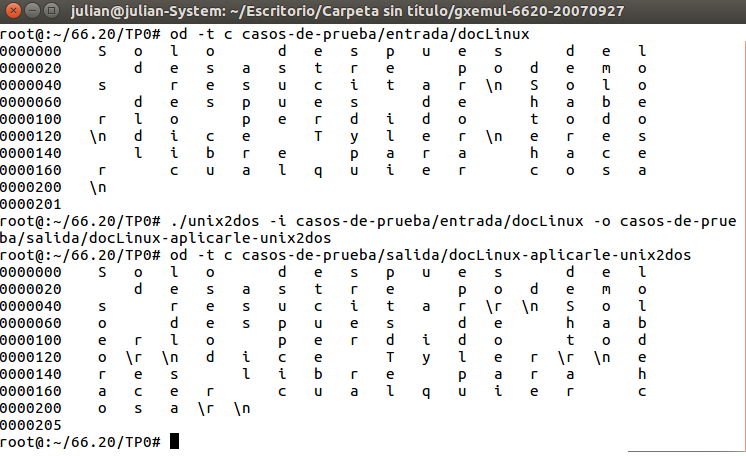
\includegraphics[width=0.8\textwidth]{/casos-prueba/docLinux-aplicarle-unix2dos-salida-archivo.png}
\caption{Prueba de transformar un archivo UNIX a Windows, utilizando archivo de entrada y salida.} \label{fig001}
\end{center}
\end{figure}

\begin{figure}[!htp]
\begin{center}
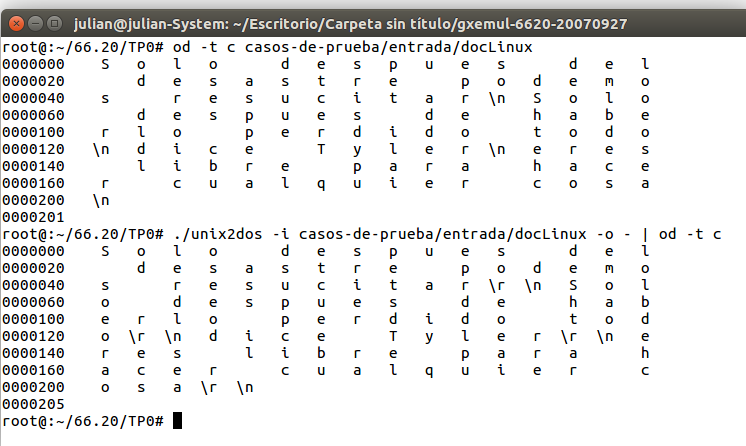
\includegraphics[width=0.8\textwidth]{/casos-prueba/docLinux-aplicarle-unix2dos-salida-estandar.png}
\caption{Prueba de transformar un arhivo UNIX a Windows, utilizando solamente archivo de entrada.} \label{fig001}
\end{center}
\end{figure}

\begin{figure}[!htp]
\begin{center}
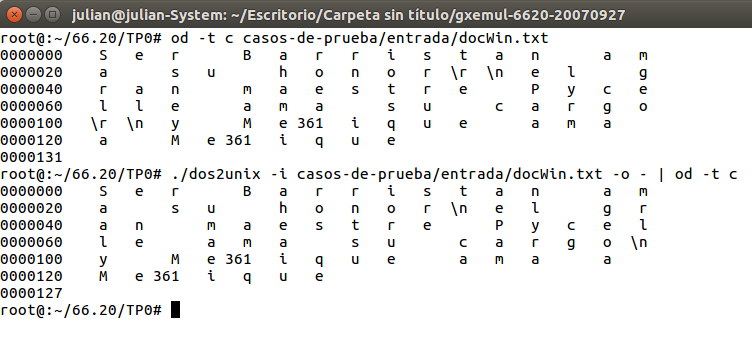
\includegraphics[width=0.8\textwidth]{/casos-prueba/docWin-aplicarle-dos2unix-salida-estandar.png}
\caption{Prueba de transformar un archivo Windows a UNIX, utilizando solo archivo de entrada.} \label{fig001}
\end{center}
\end{figure}

\begin{figure}[!htp]
\begin{center}
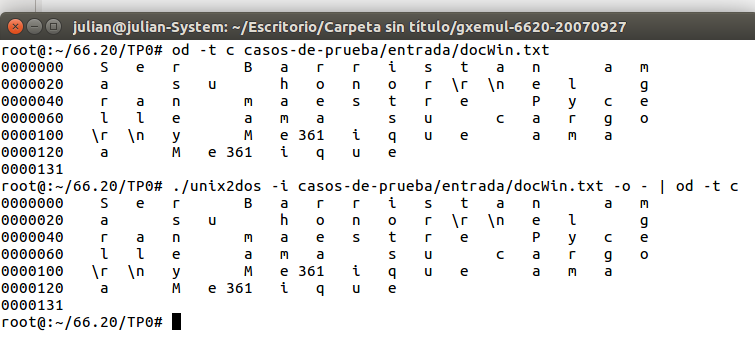
\includegraphics[width=0.8\textwidth]{/casos-prueba/docWin-aplicarle-unix2Dos-salida-estandar.png}
\caption{Prueba de transformar un archivo Windows a un archivo Windows, la salida es la misma.} \label{fig001}
\end{center}
\end{figure}

\pagebreak

\section{Código MIPS generado} 

\subsection{Código fuente assembly de unix2dos.S}

\begin{lstlisting}[language=Assembler]

	.file	1 "unix2dos.c"
	.section .mdebug.abi32
	.previous
	.abicalls
	.rdata
	.align	2
$LC0:
	.ascii	"\r\n\000"
	.align	2
$LC1:
	.ascii	"\r\000"
	.align	2
$LC2:
	.ascii	"%c\000"
	.align	2
$LC3:
	.ascii	"Error fclose: %s\n\000"
	.text
	.align	2
	.globl	processInput
	.ent	processInput
processInput:
	.frame	$fp,48,$31		# vars= 8, regs= 3/0, args= 16, extra= 8
	.mask	0xd0000000,-8
	.fmask	0x00000000,0
	.set	noreorder
	.cpload	$25
	.set	reorder
	subu	$sp,$sp,48
	.cprestore 16
	sw	$31,40($sp)
	sw	$fp,36($sp)
	sw	$28,32($sp)
	move	$fp,$sp
	sw	$4,48($fp)
	sw	$5,52($fp)
$L18:
	lw	$4,48($fp)
	la	$25,fgetc
	jal	$31,$25
	sw	$2,24($fp)
	lw	$3,24($fp)
	li	$2,-1			# 0xffffffffffffffff
	bne	$3,$2,$L20
	b	$L19
$L20:
	lw	$3,24($fp)
	li	$2,13			# 0xd
	bne	$3,$2,$L21
	lw	$4,48($fp)
	la	$25,fgetc
	jal	$31,$25
	sw	$2,24($fp)
	lw	$3,24($fp)
	li	$2,10			# 0xa
	bne	$3,$2,$L22
	lw	$4,52($fp)
	la	$5,$LC0
	la	$25,fprintf
	jal	$31,$25
	b	$L18
$L22:
	lw	$4,52($fp)
	la	$5,$LC1
	la	$25,fprintf
	jal	$31,$25
	b	$L18
$L21:
	lw	$3,24($fp)
	li	$2,10			# 0xa
	bne	$3,$2,$L25
	lw	$4,52($fp)
	la	$5,$LC0
	la	$25,fprintf
	jal	$31,$25
	b	$L18
$L25:
	lw	$4,52($fp)
	la	$5,$LC2
	lw	$6,24($fp)
	la	$25,fprintf
	jal	$31,$25
	b	$L18
$L19:
	lw	$4,48($fp)
	la	$25,fclose
	jal	$31,$25
	move	$3,$2
	li	$2,-1			# 0xffffffffffffffff
	bne	$3,$2,$L27
	la	$25,__errno
	jal	$31,$25
	lw	$4,0($2)
	la	$25,strerror
	jal	$31,$25
	la	$4,__sF+176
	la	$5,$LC3
	move	$6,$2
	la	$25,fprintf
	jal	$31,$25
	li	$2,-1			# 0xffffffffffffffff
	sw	$2,28($fp)
	b	$L17
$L27:
	lw	$3,52($fp)
	la	$2,__sF+88
	beq	$3,$2,$L28
	lw	$4,52($fp)
	la	$25,fclose
	jal	$31,$25
	move	$3,$2
	li	$2,-1			# 0xffffffffffffffff
	bne	$3,$2,$L28
	la	$25,__errno
	jal	$31,$25
	lw	$4,0($2)
	la	$25,strerror
	jal	$31,$25
	la	$4,__sF+176
	la	$5,$LC3
	move	$6,$2
	la	$25,fprintf
	jal	$31,$25
	li	$2,-1			# 0xffffffffffffffff
	sw	$2,28($fp)
	b	$L17
$L28:
	sw	$0,28($fp)
$L17:
	lw	$2,28($fp)
	move	$sp,$fp
	lw	$31,40($sp)
	lw	$fp,36($sp)
	addu	$sp,$sp,48
	j	$31
	.end	processInput
	.size	processInput, .-processInput
	.rdata
	.align	2
$LC5:
	.ascii	"version\000"
	.align	2
$LC6:
	.ascii	"help\000"
	.align	2
$LC7:
	.ascii	"input\000"
	.align	2
$LC8:
	.ascii	"output\000"
	.data
	.align	2
$LC9:
	.word	$LC5
	.word	0
	.word	0
	.word	86
	.word	$LC6
	.word	0
	.word	0
	.word	104
	.word	$LC7
	.word	1
	.word	0
	.word	105
	.word	$LC8
	.word	1
	.word	0
	.word	111
	.word	0
	.word	0
	.word	0
	.word	0
	.globl	memcpy
	.rdata
	.align	2
$LC4:
	.ascii	"i:o:hV\000"
	.align	2
$LC10:
	.ascii	"TP #0 de la materia Organizaci\303\263n de Computadoras "
	.ascii	"\n\000"
	.align	2
$LC11:
	.ascii	"Alumnos: \n\000"
	.align	2
$LC12:
	.ascii	"\tBobadilla Catalan German\n"
	.ascii	"\tDel Carril Manuel \n"
	.ascii	"\tQuino Lopez Julian \n\000"
	.align	2
$LC13:
	.ascii	"Usage: \n\000"
	.align	2
$LC14:
	.ascii	"\t%s -h \n\000"
	.align	2
$LC15:
	.ascii	"\t%s -V \n\000"
	.align	2
$LC16:
	.ascii	"\t%s [options] \n\000"
	.align	2
$LC17:
	.ascii	"Options: \n\000"
	.align	2
$LC18:
	.ascii	"\t-V, --version  Print version and quit. \n\000"
	.align	2
$LC19:
	.ascii	"\t-h, --help     Print this information. \n\000"
	.align	2
$LC20:
	.ascii	"\t-o, --output   Location of the output file. \n\000"
	.align	2
$LC21:
	.ascii	"\t-i, --input    Location of the input file. \n\000"
	.align	2
$LC22:
	.ascii	"-\000"
	.align	2
$LC23:
	.ascii	"r\000"
	.align	2
$LC24:
	.ascii	"Error archivo entrada: %s\n\000"
	.align	2
$LC25:
	.ascii	"w+\000"
	.align	2
$LC26:
	.ascii	"Error archivo salida: %s\n\000"
	.text
	.align	2
	.globl	main
	.ent	main
main:
	.frame	$fp,152,$31		# vars= 104, regs= 3/0, args= 24, extra= 8
	.mask	0xd0000000,-8
	.fmask	0x00000000,0
	.set	noreorder
	.cpload	$25
	.set	reorder
	subu	$sp,$sp,152
	.cprestore 24
	sw	$31,144($sp)
	sw	$fp,140($sp)
	sw	$28,136($sp)
	move	$fp,$sp
	sw	$4,152($fp)
	sw	$5,156($fp)
	sw	$0,32($fp)
	la	$2,$LC4
	sw	$2,36($fp)
	addu	$2,$fp,40
	la	$3,$LC9
	move	$4,$2
	move	$5,$3
	li	$6,80			# 0x50
	la	$25,memcpy
	jal	$31,$25
	sw	$0,120($fp)
	sw	$0,124($fp)
$L31:
	addu	$2,$fp,40
	sw	$0,16($sp)
	lw	$4,152($fp)
	lw	$5,156($fp)
	lw	$6,36($fp)
	move	$7,$2
	la	$25,getopt_long
	jal	$31,$25
	sw	$2,32($fp)
	lw	$3,32($fp)
	li	$2,-1			# 0xffffffffffffffff
	bne	$3,$2,$L33
	b	$L32
$L33:
	lw	$2,32($fp)
	sw	$2,132($fp)
	li	$2,104			# 0x68
	lw	$3,132($fp)
	beq	$3,$2,$L36
	lw	$3,132($fp)
	slt	$2,$3,105
	beq	$2,$0,$L45
	li	$2,86			# 0x56
	lw	$3,132($fp)
	beq	$3,$2,$L35
	b	$L43
$L45:
	li	$2,105			# 0x69
	lw	$3,132($fp)
	beq	$3,$2,$L37
	li	$2,111			# 0x6f
	lw	$3,132($fp)
	beq	$3,$2,$L40
	b	$L43
$L35:
	la	$4,$LC10
	la	$25,printf
	jal	$31,$25
	la	$4,$LC11
	la	$25,printf
	jal	$31,$25
	la	$4,$LC12
	la	$25,printf
	jal	$31,$25
	sw	$0,128($fp)
	b	$L30
$L36:
	la	$4,$LC13
	la	$25,printf
	jal	$31,$25
	lw	$2,156($fp)
	la	$4,$LC14
	lw	$5,0($2)
	la	$25,printf
	jal	$31,$25
	lw	$2,156($fp)
	la	$4,$LC15
	lw	$5,0($2)
	la	$25,printf
	jal	$31,$25
	lw	$2,156($fp)
	la	$4,$LC16
	lw	$5,0($2)
	la	$25,printf
	jal	$31,$25
	la	$4,$LC17
	la	$25,printf
	jal	$31,$25
	la	$4,$LC18
	la	$25,printf
	jal	$31,$25
	la	$4,$LC19
	la	$25,printf
	jal	$31,$25
	la	$4,$LC20
	la	$25,printf
	jal	$31,$25
	la	$4,$LC21
	la	$25,printf
	jal	$31,$25
	sw	$0,128($fp)
	b	$L30
$L37:
	lw	$4,optarg
	la	$5,$LC22
	la	$25,strcmp
	jal	$31,$25
	beq	$2,$0,$L31
	lw	$4,optarg
	la	$5,$LC23
	la	$25,fopen
	jal	$31,$25
	sw	$2,120($fp)
	lw	$2,120($fp)
	bne	$2,$0,$L31
	la	$25,__errno
	jal	$31,$25
	lw	$4,0($2)
	la	$25,strerror
	jal	$31,$25
	la	$4,__sF+176
	la	$5,$LC24
	move	$6,$2
	la	$25,fprintf
	jal	$31,$25
	b	$L31
$L40:
	lw	$4,optarg
	la	$5,$LC22
	la	$25,strcmp
	jal	$31,$25
	beq	$2,$0,$L31
	lw	$4,optarg
	la	$5,$LC25
	la	$25,fopen
	jal	$31,$25
	sw	$2,124($fp)
	lw	$2,124($fp)
	bne	$2,$0,$L31
	la	$25,__errno
	jal	$31,$25
	lw	$4,0($2)
	la	$25,strerror
	jal	$31,$25
	la	$4,__sF+176
	la	$5,$LC26
	move	$6,$2
	la	$25,fprintf
	jal	$31,$25
	li	$2,-1			# 0xffffffffffffffff
	sw	$2,128($fp)
	b	$L30
$L43:
	la	$25,abort
	jal	$31,$25
$L32:
	lw	$2,120($fp)
	bne	$2,$0,$L46
	la	$2,__sF
	sw	$2,120($fp)
$L46:
	lw	$2,124($fp)
	bne	$2,$0,$L47
	la	$2,__sF+88
	sw	$2,124($fp)
$L47:
	lw	$4,120($fp)
	lw	$5,124($fp)
	la	$25,processInput
	jal	$31,$25
	move	$3,$2
	li	$2,-1			# 0xffffffffffffffff
	bne	$3,$2,$L48
	li	$3,-1			# 0xffffffffffffffff
	sw	$3,128($fp)
	b	$L30
$L48:
	sw	$0,128($fp)
$L30:
	lw	$2,128($fp)
	move	$sp,$fp
	lw	$31,144($sp)
	lw	$fp,140($sp)
	addu	$sp,$sp,152
	j	$31
	.end	main
	.size	main, .-main
	.ident	"GCC: (GNU) 3.3.3 (NetBSD nb3 20040520)"

\end{lstlisting}

\subsection{Código fuente assembly de dos2unix.S}

\begin{lstlisting}[language=Assembler]
    
	.file	1 "dos2unix.c"
	.section .mdebug.abi32
	.previous
	.abicalls
	.rdata
	.align	2
$LC0:
	.ascii	"\n\000"
	.align	2
$LC1:
	.ascii	"\r\000"
	.align	2
$LC2:
	.ascii	"%c\000"
	.align	2
$LC3:
	.ascii	"Error fclose: %s\n\000"
	.text
	.align	2
	.globl	processInput
	.ent	processInput
processInput:
	.frame	$fp,48,$31		# vars= 8, regs= 3/0, args= 16, extra= 8
	.mask	0xd0000000,-8
	.fmask	0x00000000,0
	.set	noreorder
	.cpload	$25
	.set	reorder
	subu	$sp,$sp,48
	.cprestore 16
	sw	$31,40($sp)
	sw	$fp,36($sp)
	sw	$28,32($sp)
	move	$fp,$sp
	sw	$4,48($fp)
	sw	$5,52($fp)
$L18:
	lw	$4,48($fp)
	la	$25,fgetc
	jal	$31,$25
	sw	$2,24($fp)
	lw	$3,24($fp)
	li	$2,-1			# 0xffffffffffffffff
	bne	$3,$2,$L20
	b	$L19
$L20:
	lw	$3,24($fp)
	li	$2,13			# 0xd
	bne	$3,$2,$L21
	lw	$4,48($fp)
	la	$25,fgetc
	jal	$31,$25
	sw	$2,24($fp)
	lw	$3,24($fp)
	li	$2,10			# 0xa
	bne	$3,$2,$L22
	lw	$4,52($fp)
	la	$5,$LC0
	la	$25,fprintf
	jal	$31,$25
	b	$L18
$L22:
	lw	$4,52($fp)
	la	$5,$LC1
	la	$25,fprintf
	jal	$31,$25
	lw	$4,52($fp)
	la	$5,$LC2
	lw	$6,24($fp)
	la	$25,fprintf
	jal	$31,$25
	b	$L18
$L21:
	lw	$4,52($fp)
	la	$5,$LC2
	lw	$6,24($fp)
	la	$25,fprintf
	jal	$31,$25
	b	$L18
$L19:
	lw	$4,48($fp)
	la	$25,fclose
	jal	$31,$25
	move	$3,$2
	li	$2,-1			# 0xffffffffffffffff
	bne	$3,$2,$L25
	la	$25,__errno
	jal	$31,$25
	lw	$4,0($2)
	la	$25,strerror
	jal	$31,$25
	la	$4,__sF+176
	la	$5,$LC3
	move	$6,$2
	la	$25,fprintf
	jal	$31,$25
	li	$2,-1			# 0xffffffffffffffff
	sw	$2,28($fp)
	b	$L17
$L25:
	lw	$3,52($fp)
	la	$2,__sF+88
	beq	$3,$2,$L26
	lw	$4,52($fp)
	la	$25,fclose
	jal	$31,$25
	move	$3,$2
	li	$2,-1			# 0xffffffffffffffff
	bne	$3,$2,$L26
	la	$25,__errno
	jal	$31,$25
	lw	$4,0($2)
	la	$25,strerror
	jal	$31,$25
	la	$4,__sF+176
	la	$5,$LC3
	move	$6,$2
	la	$25,fprintf
	jal	$31,$25
	li	$2,-1			# 0xffffffffffffffff
	sw	$2,28($fp)
	b	$L17
$L26:
	sw	$0,28($fp)
$L17:
	lw	$2,28($fp)
	move	$sp,$fp
	lw	$31,40($sp)
	lw	$fp,36($sp)
	addu	$sp,$sp,48
	j	$31
	.end	processInput
	.size	processInput, .-processInput
	.rdata
	.align	2
$LC5:
	.ascii	"version\000"
	.align	2
$LC6:
	.ascii	"help\000"
	.align	2
$LC7:
	.ascii	"input\000"
	.align	2
$LC8:
	.ascii	"output\000"
	.data
	.align	2
$LC9:
	.word	$LC5
	.word	0
	.word	0
	.word	86
	.word	$LC6
	.word	0
	.word	0
	.word	104
	.word	$LC7
	.word	1
	.word	0
	.word	105
	.word	$LC8
	.word	1
	.word	0
	.word	111
	.word	0
	.word	0
	.word	0
	.word	0
	.globl	memcpy
	.rdata
	.align	2
$LC4:
	.ascii	"i:o:hV\000"
	.align	2
$LC10:
	.ascii	"TP #0 de la materia Organizaci\303\263n de Computadoras "
	.ascii	"\n\000"
	.align	2
$LC11:
	.ascii	"Alumnos: \n\000"
	.align	2
$LC12:
	.ascii	"\tBobadilla Catalan German\n"
	.ascii	"\tDel Carril Manuel \n"
	.ascii	"\tQuino Lopez Julian \n\000"
	.align	2
$LC13:
	.ascii	"Usage: \n\000"
	.align	2
$LC14:
	.ascii	"\t%s -h \n\000"
	.align	2
$LC15:
	.ascii	"\t%s -V \n\000"
	.align	2
$LC16:
	.ascii	"\t%s [options] \n\000"
	.align	2
$LC17:
	.ascii	"Options: \n\000"
	.align	2
$LC18:
	.ascii	"\t-V, --version  Print version and quit. \n\000"
	.align	2
$LC19:
	.ascii	"\t-h, --help     Print this information. \n\000"
	.align	2
$LC20:
	.ascii	"\t-o, --output   Location of the output file. \n\000"
	.align	2
$LC21:
	.ascii	"\t-i, --input    Location of the input file. \n\000"
	.align	2
$LC22:
	.ascii	"-\000"
	.align	2
$LC23:
	.ascii	"r\000"
	.align	2
$LC24:
	.ascii	"Error archivo entrada: %s\n\000"
	.align	2
$LC25:
	.ascii	"w+\000"
	.align	2
$LC26:
	.ascii	"Error archivo salida: %s\n\000"
	.text
	.align	2
	.globl	main
	.ent	main
main:
	.frame	$fp,152,$31		# vars= 104, regs= 3/0, args= 24, extra= 8
	.mask	0xd0000000,-8
	.fmask	0x00000000,0
	.set	noreorder
	.cpload	$25
	.set	reorder
	subu	$sp,$sp,152
	.cprestore 24
	sw	$31,144($sp)
	sw	$fp,140($sp)
	sw	$28,136($sp)
	move	$fp,$sp
	sw	$4,152($fp)
	sw	$5,156($fp)
	sw	$0,32($fp)
	la	$2,$LC4
	sw	$2,36($fp)
	addu	$2,$fp,40
	la	$3,$LC9
	move	$4,$2
	move	$5,$3
	li	$6,80			# 0x50
	la	$25,memcpy
	jal	$31,$25
	sw	$0,120($fp)
	sw	$0,124($fp)
$L29:
	addu	$2,$fp,40
	sw	$0,16($sp)
	lw	$4,152($fp)
	lw	$5,156($fp)
	lw	$6,36($fp)
	move	$7,$2
	la	$25,getopt_long
	jal	$31,$25
	sw	$2,32($fp)
	lw	$3,32($fp)
	li	$2,-1			# 0xffffffffffffffff
	bne	$3,$2,$L31
	b	$L30
$L31:
	lw	$2,32($fp)
	sw	$2,132($fp)
	li	$2,104			# 0x68
	lw	$3,132($fp)
	beq	$3,$2,$L34
	lw	$3,132($fp)
	slt	$2,$3,105
	beq	$2,$0,$L43
	li	$2,86			# 0x56
	lw	$3,132($fp)
	beq	$3,$2,$L33
	b	$L41
$L43:
	li	$2,105			# 0x69
	lw	$3,132($fp)
	beq	$3,$2,$L35
	li	$2,111			# 0x6f
	lw	$3,132($fp)
	beq	$3,$2,$L38
	b	$L41
$L33:
	la	$4,$LC10
	la	$25,printf
	jal	$31,$25
	la	$4,$LC11
	la	$25,printf
	jal	$31,$25
	la	$4,$LC12
	la	$25,printf
	jal	$31,$25
	sw	$0,128($fp)
	b	$L28
$L34:
	la	$4,$LC13
	la	$25,printf
	jal	$31,$25
	lw	$2,156($fp)
	la	$4,$LC14
	lw	$5,0($2)
	la	$25,printf
	jal	$31,$25
	lw	$2,156($fp)
	la	$4,$LC15
	lw	$5,0($2)
	la	$25,printf
	jal	$31,$25
	lw	$2,156($fp)
	la	$4,$LC16
	lw	$5,0($2)
	la	$25,printf
	jal	$31,$25
	la	$4,$LC17
	la	$25,printf
	jal	$31,$25
	la	$4,$LC18
	la	$25,printf
	jal	$31,$25
	la	$4,$LC19
	la	$25,printf
	jal	$31,$25
	la	$4,$LC20
	la	$25,printf
	jal	$31,$25
	la	$4,$LC21
	la	$25,printf
	jal	$31,$25
	sw	$0,128($fp)
	b	$L28
$L35:
	lw	$4,optarg
	la	$5,$LC22
	la	$25,strcmp
	jal	$31,$25
	beq	$2,$0,$L29
	lw	$4,optarg
	la	$5,$LC23
	la	$25,fopen
	jal	$31,$25
	sw	$2,120($fp)
	lw	$2,120($fp)
	bne	$2,$0,$L29
	la	$25,__errno
	jal	$31,$25
	lw	$4,0($2)
	la	$25,strerror
	jal	$31,$25
	la	$4,__sF+176
	la	$5,$LC24
	move	$6,$2
	la	$25,fprintf
	jal	$31,$25
	b	$L29
$L38:
	lw	$4,optarg
	la	$5,$LC22
	la	$25,strcmp
	jal	$31,$25
	beq	$2,$0,$L29
	lw	$4,optarg
	la	$5,$LC25
	la	$25,fopen
	jal	$31,$25
	sw	$2,124($fp)
	lw	$2,124($fp)
	bne	$2,$0,$L29
	la	$25,__errno
	jal	$31,$25
	lw	$4,0($2)
	la	$25,strerror
	jal	$31,$25
	la	$4,__sF+176
	la	$5,$LC26
	move	$6,$2
	la	$25,fprintf
	jal	$31,$25
	li	$2,-1			# 0xffffffffffffffff
	sw	$2,128($fp)
	b	$L28
$L41:
	la	$25,abort
	jal	$31,$25
$L30:
	lw	$2,120($fp)
	bne	$2,$0,$L44
	la	$2,__sF
	sw	$2,120($fp)
$L44:
	lw	$2,124($fp)
	bne	$2,$0,$L45
	la	$2,__sF+88
	sw	$2,124($fp)
$L45:
	lw	$4,120($fp)
	lw	$5,124($fp)
	la	$25,processInput
	jal	$31,$25
	move	$3,$2
	li	$2,-1			# 0xffffffffffffffff
	bne	$3,$2,$L46
	li	$3,-1			# 0xffffffffffffffff
	sw	$3,128($fp)
	b	$L28
$L46:
	sw	$0,128($fp)
$L28:
	lw	$2,128($fp)
	move	$sp,$fp
	lw	$31,144($sp)
	lw	$fp,140($sp)
	addu	$sp,$sp,152
	j	$31
	.end	main
	.size	main, .-main
	.ident	"GCC: (GNU) 3.3.3 (NetBSD nb3 20040520)"

\end{lstlisting}


\section{Conclusiones}

El trabajo práctico nos resultó interesante, no por el programa a desarrollar en sí, sino por lo que representó trabajar con el emulador GXEmul, emular la arquitectura MIPS, crear el túnel de comunicación entre el host OS (Linux, distribución Ubuntu) y el guest OS (NetBSD). Aprendimos como transferir archivos entre ambos sistemas y también ciertas cuestiones del lenguaje C con el cual no estábamos toalmente familiarizados.

\begin{thebibliography}{2}

\bibitem{lib} GetOpt library, 
\texttt{https://www.gnu.org/software/libc/manual/html_node/Example-of-Getopt.html.}

\bibitem{stack} StackOverflow, https://www.stackoverflow.com.

\end{thebibliography}

\end{document}
